\documentclass[aspectratio=1610,14pt,t]{beamer}

\usepackage{fontspec}
\newfontfamily\DejaVu{DejaVu Sans}

% Colors
\usepackage{color}
\definecolor{mainorange}{HTML}{EC811B}
\definecolor{lightgrey}{HTML}{888888}
\definecolor{almostwhite}{HTML}{FEFEFE}

% Video support
\usepackage{multimedia}

% Syntax highlighting
\usepackage{minted}
\usepackage{alltt}
\newcommand\hi[1]{{\color{mainorange} \textbf{#1}}}

\usepackage{wasysym}

% Custom unicode symbols
\usepackage{newunicodechar}
\newcommand\Warning{%
 \makebox[1.4em][c]{%
 \makebox[0pt][c]{\raisebox{.1em}{\small!}}%
 \makebox[0pt][c]{\color{red}\Large$\bigtriangleup$}}}%

\newunicodechar{⚠}{\Warning}

% Theme
\usetheme[%
  subsectionpage=progressbar,
  numbering=fraction,
  progressbar=foot,
]{metropolis}

% Customization
\usepackage{pagecolor}
\setbeamertemplate{section in toc}[sections numbered]
\setbeamerfont{title}{size=\fontsize{30}{30}}
\setbeamerfont{block title}{size=\large}
\newcommand\sep{\textcolor{lightgrey}{\rule{\linewidth}{0.05mm}}}

% Positioning
% https://tex.stackexchange.com/a/34929/13059
\def\Put(#1,#2)#3{\leavevmode\makebox(0,0){\put(#1,#2){#3}}}

% Meta
\title{Embedded Rust}
\date{2020-06-18}
\author{Raphael Nestler (@rnestler), Noah Hüsser (@Yatekii)}
\institute{Rust Zürichsee Meetup}

\begin{document}

\pgfdeclareimage[width=\paperwidth]{bg}{background-dark.pdf}
\pagecolor{almostwhite}  % Prevent speakerdeck from optimizing away the bg color
\usebackgroundtemplate{\pgfuseimage{bg}}
\maketitle

% ----------------------------------------------------------------- %

\begin{frame}[c]{println!("\{:?\}", rnestler)}
  Hi! I'm Raphael (@rnestler).

  \pause I live in Rapperswil

  \pause I work at Sensirion ({\small \url{https://sensirion.com}}).

  \pause I'm a founding member of Coredump\\hackerspace ({\small \url{https://coredump.ch}}).
\end{frame}

\begin{frame}[c]{println!("\{:?\}", yatekii)}
  Hi! I'm Noah (@Yatekii).

  \pause I live in Lenzburg

  \pause I work at Technokrat ({\small \url{https://technokrat.ch/}}).

  \pause I started the probe-rs project ({\small \url{https://probe-rs}}).
\end{frame}

% ----------------------------------------------------------------- %

\begin{frame}[plain,noframenumbering]
  \frametitle{Outline}
  \setcounter{tocdepth}{1}
  \tableofcontents
\end{frame}

% ----------------------------------------------------------------- %

\pgfdeclareimage[width=\paperwidth]{bg}{background-light.pdf}
\usebackgroundtemplate{\pgfuseimage{bg}}

\section{Embedded Programming}

\begin{frame}[c]{What is an \emph{Embedded System}?}
  \begin{quote}
    A combination of computer hardware and software, and perhaps
    additional mechanical or other parts, designed to perform a dedicated
    function.
  \end{quote}
  Michael Barr. ``Embedded Systems Glossary''\footnote{\tiny\url{https://barrgroup.com/Embedded-Systems/Glossary-E\#embedded\_system}}
\end{frame}

\begin{frame}[c]{What is embedded programming?}
  \begin{itemize}
    \item Dedicated, not general purpose, µC system
    \item<1-> Baremetal
    \item<1-> Low-Level
    \item<2-> For this talk: Bare metal on Cortex-M MCUs
  \end{itemize}
\end{frame}

\begin{frame}[c]{Why do they say it's hard?}
  \begin{itemize}
    \item Harsh environment (No OS which protects you)
    \item Resource constrained (Remember dedicated?)
    \item Non-standard, Non-OSS toolchain
    \item Hard realtime requirements
    \item \ldots
  \end{itemize}
\end{frame}

\begin{frame}[c]{What does it mean for Rust?}
  \centering
  
\includegraphics[height=0.8\textheight]{img/no-std-gandalf.jpg}
\end{frame}


\begin{frame}[c]{Why is Rust awesome for it?}
  \begin{itemize}
    \item Zero cost abstractions!
    \item Provides safety at compiler level, not OS
    \item Expressive type system to encode constraints
  \end{itemize}
\end{frame}

\section{State of Embedded in 2020}
\begin{frame}[c]{The compiler}
  \begin{itemize}
    \item \texttt{const fn}
    \item \texttt{core::future::Future}
    \item \texttt{alloc} crate is stable
    \item \texttt{MaybeUninit<T>}: Fixes undefined behavior
  \end{itemize}
\end{frame}

\begin{frame}[c]{The compiler}
  \includegraphics[height=0.8\textheight]{img/did-i-forget-something.jpg}
\end{frame}

\begin{frame}[c]{\texttt{async} / \texttt{await} of course}

  \begin{quote}
    The \texttt{.await} is over, \texttt{async fn}s are here
  \end{quote}

  $\rightarrow$ We'll get to it
\end{frame}

\subsection{\texttt{const fn}}

\begin{frame}{Constant Fun!}
  \begin{columns}[t,onlytextwidth]
    \column{.4\textwidth}
    \begin{figure}
    
\includegraphics[width=\textwidth]{img/const-all-the-fn.jpg}
    \end{figure}
    \column{.6\textwidth}
    \begin{itemize}
      \item Stabilized at the end of 2018
      \item Tons of functions got const during 2019
      \item More functions from libcore
      \item More features (destructuring, bindings, assignment, \ldots)
    \end{itemize}
  \end{columns}
\end{frame}

\begin{frame}[c,fragile]{Constant Fun Example}
An example from the lin-bus crate\footnote{\url{https://github.com/Sensirion/lin-bus-rs/blob/e89739e326daf091803373419a4d60d0888422fc/src/frame.rs}}
  \begin{minted}[fontsize=\footnotesize]{rust}
/// Calculate the PID from an ID.
/// P0 = ID0 ^ ID1 ^ ID2 ^ ID4
/// P1 = ¬(ID1 ^ ID3 ^ ID4 ^ ID5)
const fn from_id_const(id: u8) -> PID {
    // count parity bits and check if they are even / odd
    let p0 = (id & 0b1_0111).count_ones() as u8 & 0b1;
    let p1 = ((id & 0b11_1010).count_ones() as u8 + 1) & 0b1;
    PID(id | (p0 << 6u8) | (p1 << 7u8))
}
  \end{minted}
\end{frame}

\begin{frame}[c,fragile]{Less Constant Fun Example}
  Saw the problem?\pause
  \begin{minted}[fontsize=\footnotesize]{rust}
pub fn from_id(id: u8) -> PID {
    assert!(id < 64, "ID must be less than 64");
    PID::from_id_const(id)
}
  \end{minted}
  \pause Workaround
  \begin{minted}[fontsize=\footnotesize]{rust}
  // check that id < 64. Compile error during const evaluation
  // and panic on debug build
  let _: u8 = id + 192;
  \end{minted}
\end{frame}

\begin{frame}{Constant Future}
  What is missing?
  \begin{itemize}
    % Important to have compile time assertions, think static_assert in C++
    \item Panicking in constants\footnote{\url{https://github.com/rust-lang/rust/issues/51999}}
    % Implementation is here, but design not finalized. You can use it on nightly.
    \item Const generics\footnote{\url{https://github.com/rust-lang/rust/issues/44580}}
  \end{itemize}
\end{frame}

\subsection{Other News}

\begin{frame}[c]{New Platform Support}
  \begin{itemize}
    \item AVR basic support got merged\footnote{\url{https://github.com/rust-lang/rust/pull/69478}} \footnote{\url{https://github.com/rust-lang/rust/issues/44052}}
    \item New ARM targets: thumbv7neon-linux-\{androideabi,gnueabihf\}, armv\{6/7\}-unknown-freebsd-gnueabihf, aarch64-unknown-none-*
    \item New RISC-V targets: riscv64imac-unknown-none-elf, riscv64gc-unknown-none-elf, riscv32i-unknown-none-elf
    \item Sony PSP support\footnote{\url{https://github.com/rust-lang/rust/pull/72062}}
  \end{itemize}
\end{frame}

\begin{frame}[c]{RTFM $\rightarrow$ RTIC}
  \begin{itemize}
    \item RTFM got renamed $\rightarrow$ RTIC\footnote{\url{https://rtic.rs/0.5/book/en/migration_rtic.html}}
    \item Examples: https://github.com/coredump-ch/nixie-counter/tree/master/firmware/
  \end{itemize}
\end{frame}

\subsection{Embedded HAL}

\begin{frame}[c]{What is the Embedded HAL?}
  \begin{itemize}
  \item Unified interface to the same HW functionality which has different
    interfaces
  \item Higher level crates (drivers) are write once use always
  \item Nice examples: shtc3
    driver\footnote{\url{https://github.com/dbrgn/shtcx-rs}} developed and
    debugged on a  Raspberry Pi and used with an STM32
  \end{itemize}
\end{frame}

\begin{frame}[c]{SHTC3 Driver as Example}
  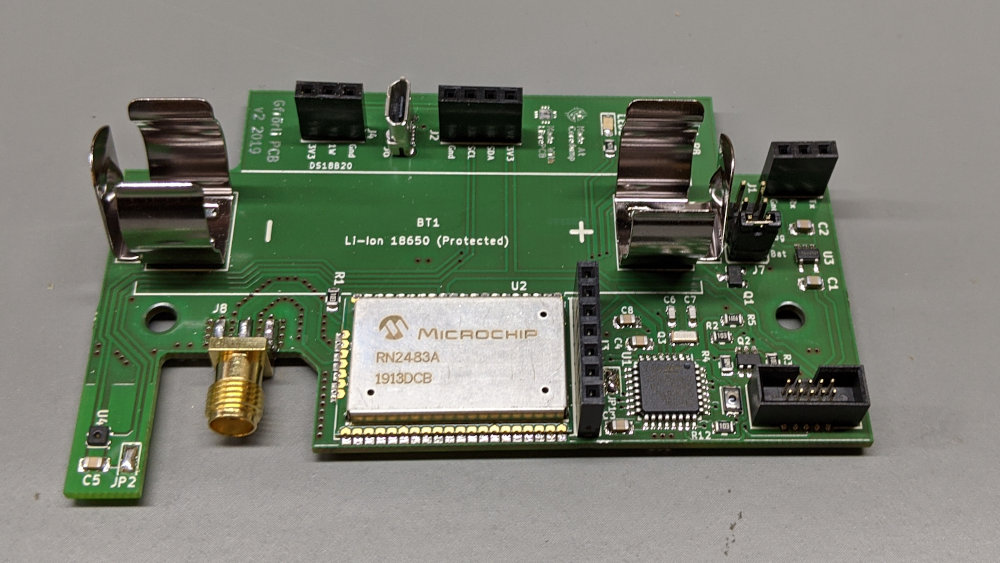
\includegraphics[height=0.8\textheight]{./img/gfroerli.jpg}
\end{frame}

\begin{frame}[c]{SHTC3 Driver as Example}
\movie[autostart,loop]{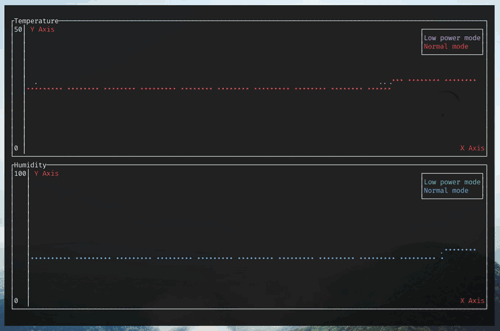
\includegraphics[height=0.8\textheight]{./img/shtc3-monitor-0.png}}{./img/shtc3-monitor.mp4}
\end{frame}

\begin{frame}[c]{Embedded HAL --- Challanges / Future}
  \begin{itemize}
  \item It's hard to define traits which work everywhere
  % Single vs. multi byte transfer, DMA? SPI CS? Own the HW device?:w

  \item How to define async traits?
  \item Ecosystem needs to move as a whole on breaking changes
  \item 1.0 Release planed\footnote{\url{https://github.com/rust-embedded/embedded-hal/issues/177}}
  \end{itemize}
\end{frame}

\subsection{async on embedded}
\begin{frame}[c]{async --- Some Background}
  \begin{itemize}
    \item async/await landed in stable Rust 1.39\footnote{\url{https://blog.rust-lang.org/2019/11/07/Async-await-stable.html}}
    \item In February 2020 Ferrous Systems started blogging about bringing it
      to embedded\footnote{\url{https://ferrous-systems.com/blog/embedded-async-await/}}
      \footnote{\url{https://ferrous-systems.com/blog/async-on-embedded/}}
    \item Since Rust 1.44 usable on \texttt{no\_std}
      \footnote{\url{https://ferrous-systems.com/blog/stable-async-on-embedded/}}
  \end{itemize}
\end{frame}

\begin{frame}[c]{async --- What is it Even?}
  \begin{itemize}
    \item Mostly syntactic suger for a state machine
    \item Useful for concurrent waiting
  \end{itemize}
\end{frame}

% This is massively oversimplified. In reality we have generic Futures and pass
% a context with the wake function to signal that the Future should be polled
% again.
\begin{frame}[c,fragile]{async --- State Machine}
  \begin{columns}[t,onlytextwidth]
  \column{.6\textwidth}
  \begin{minted}[fontsize=\small]{rust}
async fn foo() -> u8 {
    1
}
async fn bar(a: u8) -> u8 {
    a + 2
}
async fn f() -> u8 {
    let a = foo().await;
    bar(a).await
}
	\end{minted}
  \pause\column{.4\textwidth}
  \begin{minted}[fontsize=\small]{rust}
enum Future {
    Ready(u8),
    Pending,
}

enum State {
    Foo,
    Bar(u8),
    Done(u8),
}
  \end{minted}
	\end{columns}
\end{frame}

\begin{frame}[c,fragile]{async --- State Machine}
  \begin{minted}[fontsize=\small]{rust}
fn f_desugared(state: State) -> State {
    match state {
        State::Foo => match foo_() {
            Future::Ready(a) => State::Bar(a),
            Future::Pending => State::Foo,
        },
        State::Bar(a) => match bar_(a) {
            Future::Ready(b) => State::Done(b),
            Future::Pending => State::Bar(a),
        }
        State::Done(b) => State::Done(b)
    }
}
  \end{minted}
\end{frame}

\begin{frame}[c]{async --- Why on Embedded?}
  \begin{itemize}
    \item Most embedded systems are event driven $\rightarrow$ Most code is
      \emph{awaiting} events.
    \item Embedded systems may want to save power $\rightarrow$ Sleep whenever
      possible.
		\item We often need to wait for peripherals / IO
  \end{itemize}
\end{frame}

\begin{frame}[c,fragile]{async --- A blocking blinky}
  \begin{minted}[fontsize=\footnotesize]{rust}
fn main() -> ! {
    let mut led = Led::new();
    let mut timer = Timer::new();

    loop {
        led.on();
        timer.delay_ms(1_000);
        led.off();
        timer.delay_ms(1_000);
    }
}
  \end{minted}
\end{frame}

\begin{frame}[c,fragile]{async --- A async blinky}
  \begin{minted}[fontsize=\footnotesize]{rust}
fn main() -> ! {
    let mut led = Led::new();
    let mut timer = Timer::new();

    // `block_on` runs the future (`async` block) to completion
    task::block_on(async {
        loop {
            led.on();
            timer.wait(Duration::from_secs(1)).await;
            // ^ suspends the task for one second
            led.off();
            timer.wait(Duration::from_secs(1)).await;
        }
    })
}
  \end{minted}
\end{frame}



\begin{frame}[c]{async --- embrio-rs\footnote{\url{https://github.com/Nemo157/embrio-rs}}}
  \begin{itemize}
    \item Playground for async on \texttt{no\_std}
    \item Provides a custom async desugaring via a proc macro
    \item Not actively developed anymore according to author\footnote{\url{https://www.reddit.com/r/rust/comments/f0ckiv/bringing_asyncawait_to_embedded_rust/fgwh6ij/}}
    \item Works very nice on the NRF51
    \item Used in the Polymer mechanical keyboard firmware\footnote{\url{https://josh.robsonchase.com/rest-of-the-keyboard/}}
  \end{itemize}
\end{frame}

\begin{frame}[c]{async --- The \texttt{Future}}
  \begin{itemize}
    % Maybe one for Cortex-M?
    \item Reusable executors?
    % On single core just disable all interrupts in critical sections
    \item Thread safety with interrupts?
    \pause\item RTIC may provide a solution for that {\DejaVu ☺}
  \end{itemize}
\end{frame}

\begin{frame}[c]{More Resources}
  \begin{itemize}
    \item The Rust Embedded WG Blog\footnote{\url{https://rust-embedded.github.io/blog/}}
    \item The Rust Embedded Book\footnote{\url{https://docs.rust-embedded.org/book/}}
    \item The Discovery book\footnote{\url{https://docs.rust-embedded.org/discovery/index.html}}
    \item Awesome Embedded Rust\footnote{\url{https://github.com/rust-embedded/awesome-embedded-rust}}
  \end{itemize}
\end{frame}

\section{probe-rs}

\begin{frame}[c]{Embedded Development}
  \begin{itemize}
    % On an x86 target you can load the program directly from disk to RAM from with in your os.
    % Where you also coded, compiled and debugged your program.
    % You get convenient tools for output and interaction such as the commandline, a debugger or even a webbrowser.
    \item Software is written on a host instead of the target.
    % On a microchip we have no such feedback.
    % We develop the software, flash it to the microchip with a magic tool (at least to many folks it is)
    % and hope it runs properly. Oftentimes we have to measure HW signals with some special equippment.
    \item The microchip has no direct feedback.
    % We need a tool to talk with the chip. We somehow need our host to talk to the microchip.
    % To download the binary, to run a debugger and to do custom interaction.
    % Interfaces exist, but the PC doesn't understand them. Similar to an SPI peripheral and an SPI driver,
    % We need to write the driver for those interfaces. SWD and JTAG.
    \item A middleman is needed (soft- \& hardware).
    % This magic tool you always used but never really looked into is probe-rs, like many others.
    \item probe-rs
  \end{itemize}
  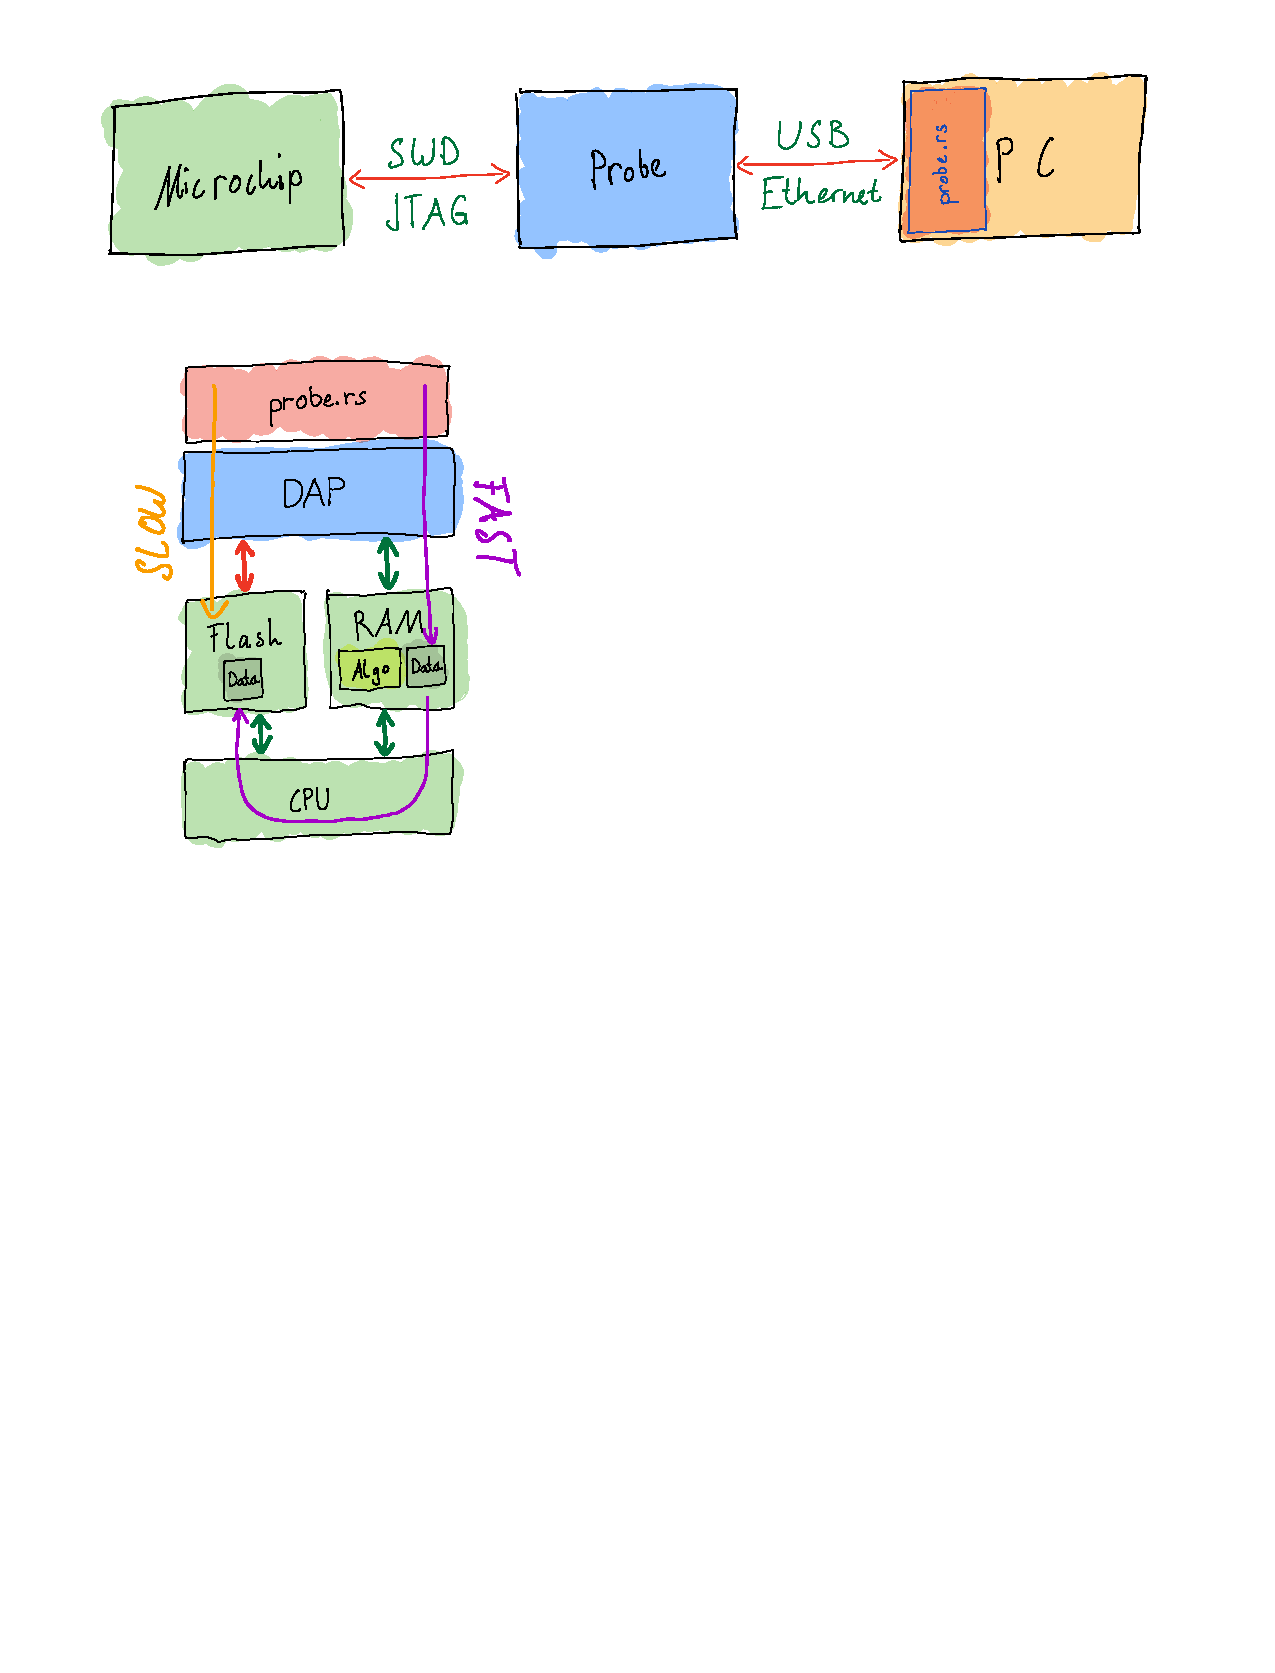
\includegraphics[trim=0 23cm 0 0, clip, height=0.4\textheight]{./img/probe-chain.pdf}
\end{frame}

\begin{frame}[c]{probe-rs!}
  \begin{itemize}
    \item Rust Library
    \item Easy to use
    \item Unified interface
    \item Developed on Github
    \item Talks to ARM and RISC-V cores (for now)
    \item Supports CMSIS-DAP, ST-Link, J-Link
  \end{itemize}
\end{frame}

\begin{frame}[c]{Current State}
  \begin{itemize}
    \item Memory Access (read, write)
    \item CPU Manipulation (run, halt, step, reset, etc.)
    \item Breakpoints (set, reset)
    \item Flashing (ELF, BIN, HEX)
  \end{itemize}
\end{frame}

\begin{frame}[c,fragile]{Memory Access}
  \begin{minted}[fontsize=\small]{rust}
    use probe_rs::Session;
    use probe_rs::MemoryInterface;

    let mut session = Session::auto_attach("nrf52")?;
    let mut core = session.core(0)?;

    // Read a single 32 bit word.
    let word = core.read_word_32(0x2000_0000)?;
  \end{minted}
\end{frame}

\begin{frame}[c,fragile]{CPU Control}
  \begin{minted}[fontsize=\small]{rust}
    use probe_rs::Session;
    use probe_rs::MemoryInterface;

    let mut session = Session::auto_attach("nrf52")?;
    let mut core = session.core(0)?;

    // Reset the CPU.
    core.reset()?;
  \end{minted}
\end{frame}

\begin{frame}[c,fragile]{Breakpoint Manipulation}
  \begin{minted}[fontsize=\small]{rust}
    use probe_rs::Session;
    use probe_rs::MemoryInterface;

    let mut session = Session::auto_attach("nrf52")?;
    let mut core = session.core(0)?;

    // Set a breakpoint.
    core.set_hw_breakpoint(0x1500_2000)?;
  \end{minted}
\end{frame}

\begin{frame}[c,fragile]{Flash Algorithms}
  \begin{columns}[t,onlytextwidth]
    \column{.7\textwidth}
    \begin{itemize}
      \item Used for fast flashing
      \item Used to circumvent slow flash access
      \item Small program loaded into RAM
      \item Copies data from RAM to Flash
      \item CMSIS-Packs
      \begin{itemize}
        \item ARM standard
        \item thousands of available targets
      \end{itemize}
    \end{itemize}
    \column{.3\textwidth}
    \begin{figure}
      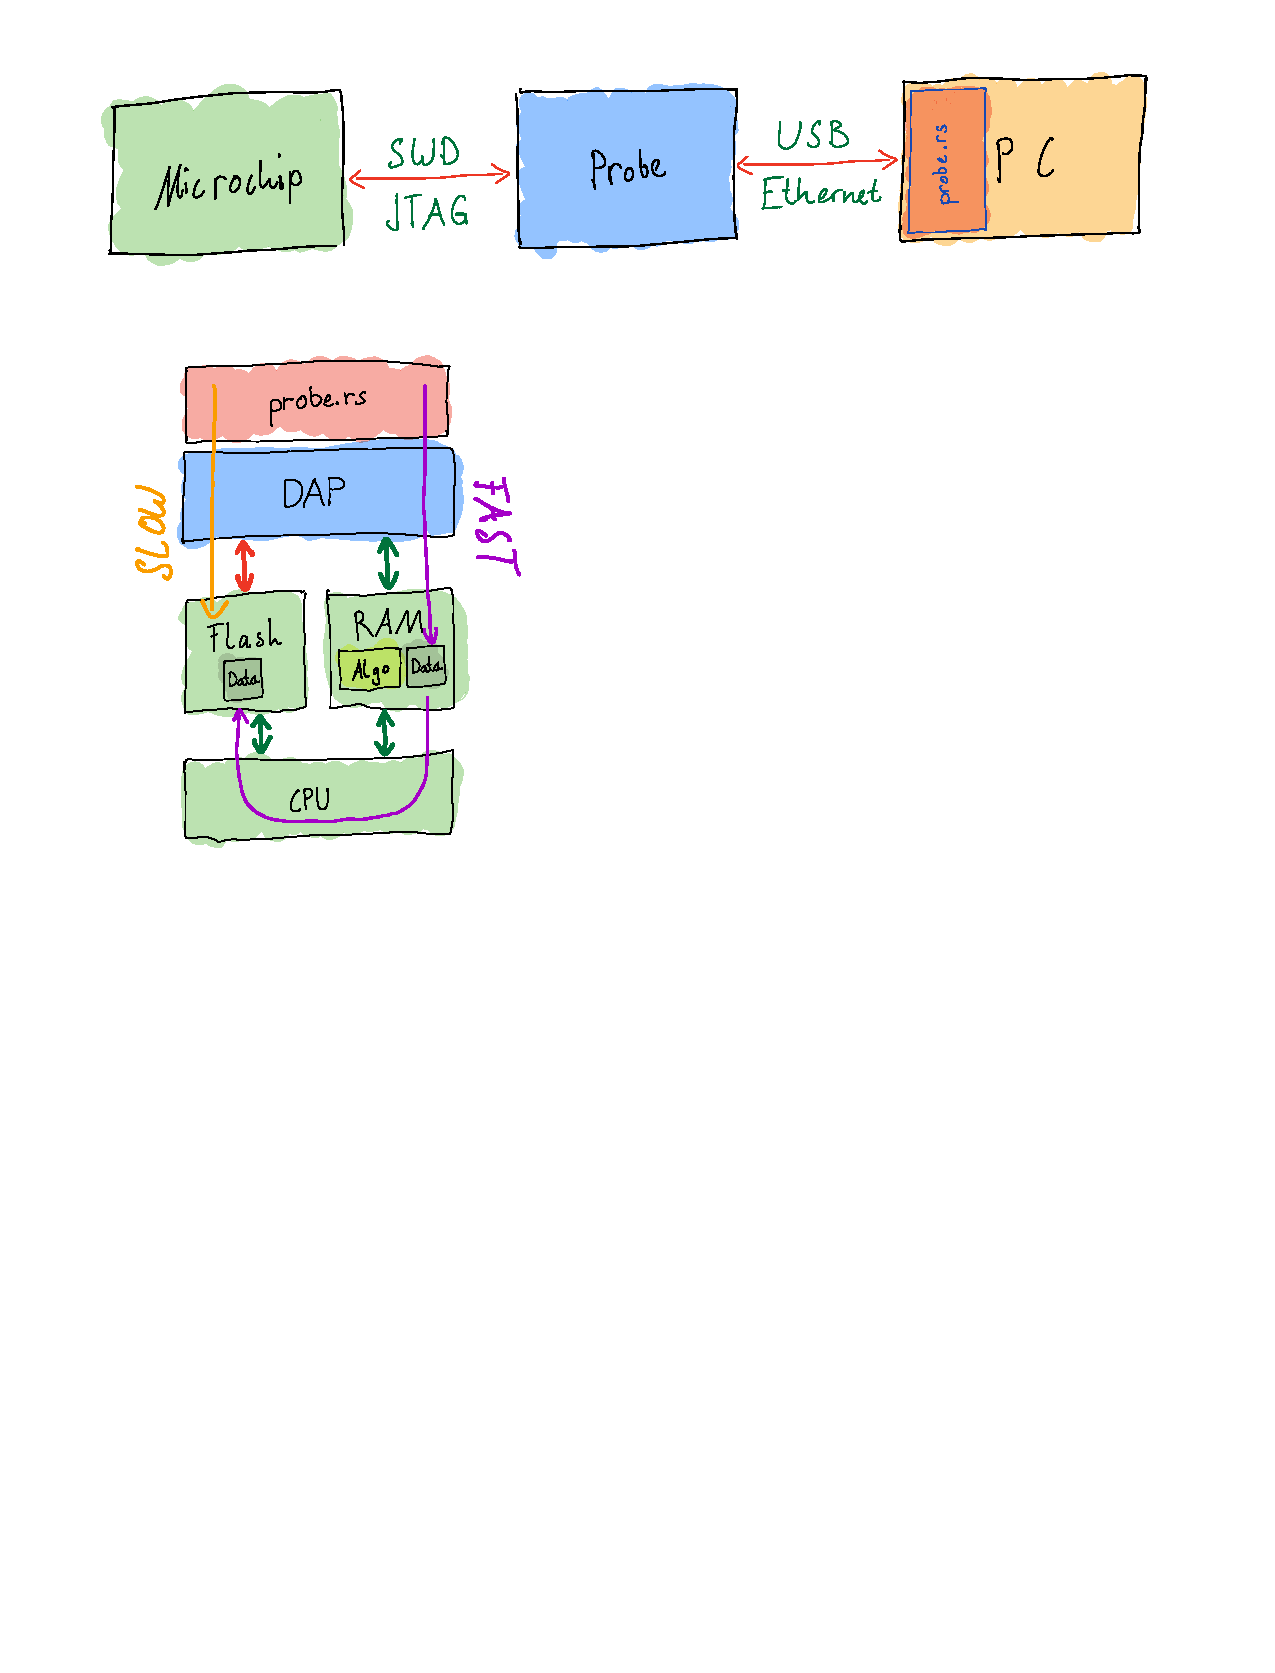
\includegraphics[trim=2cm 13cm 0 6cm, clip, width=12cm]{./img/probe-chain.pdf}
    \end{figure}
  \end{columns}
\end{frame}

\begin{frame}[c,fragile]{cargo flash}
  \begin{itemize}
    \item slim cargo plugin
    \item for flashing targets
    \item to jumpstart in a project
    \item https://github.com/probe-rs/cargo-flash
  \end{itemize}
\end{frame}

\begin{frame}[c,fragile]{cargo embed}
  \begin{itemize}
    \item fat client embedded toolkit
    \item flashing
    \item RTT
    \item GDB
    \item more?
    \item highly configurable
    \item https://github.com/probe-rs/cargo-embed
  \end{itemize}
\end{frame}

\section{probe\_rs.await?;}

\begin{frame}[c,fragile]{VSCode}
  \begin{itemize}
    \item VSCode plugin
    \item Microsoft DAP
    \item no GDB required
    \item Modern, extensive API (JSON)
    \item async
    \item working, with limitations
    \item https://github.com/probe-rs/vscode
  \end{itemize}
\end{frame}

\begin{frame}[c,fragile]{ITM}
  \begin{itemize}
    \item powerful data streaming from the target
    \item ISR events
    \item memory access events
    \item custom binary data
    \item working, not on master yet
    \item https://github.com/probe-rs/probe-rs/pull/145
  \end{itemize}
\end{frame}

\begin{frame}[c,fragile]{Custom Hooks}
  \begin{itemize}
    \item use CMSIS-Pack hooks
    \item uses custom WASM format
    \item poc, no PR yet
  \end{itemize}
\end{frame}

\begin{frame}[c,fragile]{rs-probe}
  \begin{itemize}
    \item open source probe
    \item pure rust firmware
    \item extremely fast (500 Mbit/s)
    \item uses standard ARM API
    \item can stream DAP, ITM and UART data
    \item https://github.com/korken89/hs-probe
  \end{itemize}
\end{frame}

\begin{frame}[c]{Contribute}
  \begin{itemize}
    \item https://probe.rs
    \item https://github.com/probe-rs/probe-rs
    \item \#probe-rs:matrix.org on Matrix
    \item Questions \& Bugreports very welcome
    \item PRs very welcome
  \end{itemize}
\end{frame}

% ----------------------------------------------------------------- %

{
\setbeamertemplate{footline}{}
\pgfdeclareimage[width=\paperwidth]{bg}{background-inverted.pdf}
\usebackgroundtemplate{\pgfuseimage{bg}}
\begin{frame}[standout]
  \begin{centering}
    {\Huge Thank you!}\\
    {\normalsize \url{https://coredump.ch}}\\
    {\normalsize \url{https://technokrat.ch/}}\\
  \end{centering}
  {\small Slides: \url{https://github.com/rust-zurichsee/meetups/}}\\
  \vspace{3cm}
\end{frame}
}


\setbeamertemplate{section in toc}[sections numbered]
\pgfdeclareimage[width=\paperwidth]{bg}{background-light.pdf}
\usebackgroundtemplate{\pgfuseimage{bg}}
\appendix
\section{\appendixname}
\frame{\tableofcontents}
\subsection{Alloc crate}

\begin{frame}[c]{alloc crate}
  \begin{itemize}
    \item alloc allows you to use a subset of std (e.g. \texttt{Vec, Box, Arc})
      in \texttt{\#![no\_std]} environments if the environment has access to
      heap memory allocation.\footnote{\url{https://github.com/rust-lang/rfcs/blob/master/text/2480-liballoc.md}}
    \item You need to define a \texttt{\#[global\_allocator]}\footnote{\url{https://doc.rust-lang.org/stable/std/alloc/\#the-global\_allocator-attribute}}
    \item Check out \url{https://crates.io/crates/alloc-cortex-m}
  \end{itemize}
\end{frame}

\subsection{svd2rust}

\begin{frame}[c]{svd2rust}
  \begin{itemize}
    \item Every Cortex-M μC vendor must provide an SVD (System View
      Descriptions) file
    \item SVD is an XML standard to describe peripheral registers
    \item svd2rust\footnote{\url{https://github.com/rust-embedded/svd2rust}}:
      Generate Rust register maps (structs) from SVD files
  \end{itemize}
\end{frame}

\end{document}
